%%% template.tex
%%%
%%% This LaTeX source document can be used as the basis for your technical
%%% paper or abstract. Intentionally stripped of annotation, the parameters
%%% and commands should be adjusted for your particular paper - title,
%%% author, article DOI, etc.
%%% The accompanying ``template.annotated.tex'' provides copious annotation
%%% for the commands and parameters found in the source document. (The code
%%% is identical in ``template.tex'' and ``template.annotated.tex.'')

\documentclass[]{acmsiggraph}
\usepackage{algorithm}
\usepackage[noend]{algpseudocode}
\TOGonlineid{45678}
\TOGvolume{0}
\TOGnumber{0}
\TOGarticleDOI{0}
\TOGprojectURL{}
\TOGvideoURL{}
\TOGdataURL{}
\TOGcodeURL{}
\usepackage{color}
%\definecolor{red}{rgb}{0.9, 0.17, 0.31}
\usepackage{multirow}
\usepackage{subfig}
\usepackage{xcolor}
\usepackage{lipsum}
\usepackage{listings}
\usepackage{graphicx}
\usepackage{glsllst} % My own package providing markup listing for glsl
\usepackage{rmlst}   % My own package providing markup listing for renderman
\usepackage{amsmath}
\usepackage{hyperref}

\lstset{
	backgroundcolor=\color[rgb]{0.95, 0.95, 0.95},
	tabsize=3,
	%rulecolor=,
	basicstyle=\footnotesize\ttfamily,
	upquote=true,
	aboveskip={1.5\baselineskip},
	columns=fixed,
	showstringspaces=false,
	extendedchars=true,
	breaklines=true,
	prebreak = \raisebox{0ex}[0ex][0ex]{\ensuremath{\hookleftarrow}},
	frame=none,
	aboveskip=15pt,
	belowskip=8pt,
	captionpos=t,
	showtabs=false,
	showspaces=false,
	showstringspaces=false,
	identifierstyle=\ttfamily,
	%keywordstyle=\color{red}\bfseries,
	%keywordstyle=[1]\bfseries\color{syntaxBlue},
	%keywordstyle=[2]\bfseries\color{syntaxRed},
	%keywordstyle=[3]\color{blue}\bfseries,
	%keywordstyle=[4]\bfseries\color{syntaxBlue},
	commentstyle=\color[rgb]{0.082,0.639,0.082},
	keywordstyle=[1]\bfseries\color[rgb]{0,0,0.75},
	keywordstyle=[2]\bfseries\color[rgb]{0.5,0.0,0.0},
	keywordstyle=[3]\bfseries\color[rgb]{0.127,0.427,0.514},
	keywordstyle=[4]\bfseries\color[rgb]{0.4,0.4,0.4},
	stringstyle=\color[rgb]{0.639,0.082,0.082},
}

\title{Masterclass Assignment: Real-time Global Illumination}

\author{Joe Withers\thanks{e-mail: joewithers96@gmail.com}}
\pdfauthor{Joe Withers}

\keywords{rendering}

\begin{document}

%% \teaser{
%%   \includegraphics[height=1.5in]{images/sampleteaser}
%%   \caption{Spring Training 2009, Peoria, AZ.}
%% }

\maketitle

\begin{abstract}
This document details the approach I took to complete the Masterclass assignment, evaluates the results, and lists possible improvements I could make in the future.
\end{abstract}
%\keywordlist
%\TOGlinkslist

\section{Introduction}
For this assignment I decided to implement the technique \textit{Interactive Indirect Illumination using voxel cone tracing} \cite{crassinneyretsainzgreeneisemann2011}, commonly referred to as VXGI, to achieve realtime global illumination. This technique achieves real-time global illumination rendering the directly illuminated scene geometry into a three-dimensional texture, which can be sampled in a deferred shading pass using cone tracing to calculate accurate indirect diffuse and specular lighting terms.

\section{Method}
I used C++ and OpenGL for this assignment, utilising the NCCA Graphics Library NGL \cite{ngl} to interact with OpenGL, and Qt5 to create the user interface. I based my implementation around a demo of the Sponza atrium using NGL \cite{pbrSponza}, that although is quite old, saved me from spending a lot of time writing a grouped Wavefront OBJ and MTL file parser. I extended upon this demo by converting it to use deferred shading, which is necessary for VXGI and other post process effects, using tutorial material from LearnOpenGL \cite{learnDeferred}.

The first step of implementing VXGI was to create a voxelized representation of the albedo and surface normal information in the scene. The method used in the source material \cite{crassinneyretsainzgreeneisemann2011} is explained in great detail in an OpenGL Insights chapter titled \textit{Octree-Based Sparse Voxelization Using the GPU Hardware Rasterizer} \cite{crassingreen2012}, but the basic concept is as followed:
\begin{enumerate}
	\item Generate three projection matrices for orthogonal projections, covering the scene geometry equally, and aligned to each of the coordinate axes.
	\item Draw the scene with depth testing disabled, ensuring fragments are generated for every triangle.
	\item For each triangle, determine which of the coordinate axes is most aligned with the surface normal, thus generating the maximum number of fragments when transformed using the corresponding projection matrix for that axis.
	\item Using either the NVIDIA OpenGL extension \textit{GL CONSERVATIVE RASTERIZATION NV}, or a geometry shader, enlarge each triangle so that fragments are generated regardless of whether it covers a pixels center. This helps to reduce 'cracks' in the voxelisation on surfaces that are angled away from the coordinate axes.
	\item Using the fragment coordinates, depth, and the axis chosen in step 3, infer the texel coordinate that the fragment corresponds to in the target 3D textures. Store the fragment albedo and normal information in 3D textures using a moving average.
\end{enumerate}
Whilst this technique is somewhat easy to explain, I had not previously used the required Image Load/Store commands so I referred to an implementation I found on GitHub \cite{voxelization} to guide me on the OpenGL side of things.

The next step was to inject the scene's emissive values into a 3D texture. This is achieved by raytracing towards the light, for each of the non-transparent texels in the voxelised textures. This is where my implementation differs from the source material \cite{crassinneyretsainzgreeneisemann2011} as I opted to use a dense 3D texture as opposed to a sparse voxel octree. Whilst this was significantly easier to set up, it also severly impacts the speed at which raytracing can be performed through this 3D texture (See Figure~\ref{figure:performance} for performance metrics). The source material \cite{crassinneyretsainzgreeneisemann2011} also details a method for mip-mapping this texture anisotropically along each of the coordinate axes, however I opted to use OpenGL's \lstinline{genMipMaps} method to save time.

The final step was to implement cone tracing in the deferred shading pass. This pass calculates the indirect light contribution, specular lobe contribution, and also soft shadows.


\begin{figure}[htbp]
  \centering
 \subfloat[Specular Cone]{\includegraphics[width=0.45\linewidth]{images/specularCone}}
 \hfill
 \subfloat[Diffuse Indirect Cones]{\includegraphics[width=0.45\linewidth]{images/indirectCones}}
 \caption{A side by side comparison of different render effects is always a good idea to demonstrate a choice of parameters or design of your shader. These were appropriated from \cite{Villegas2016}.}
\end{figure}

\section{Results}

\begin{figure}[htbp]\centering
 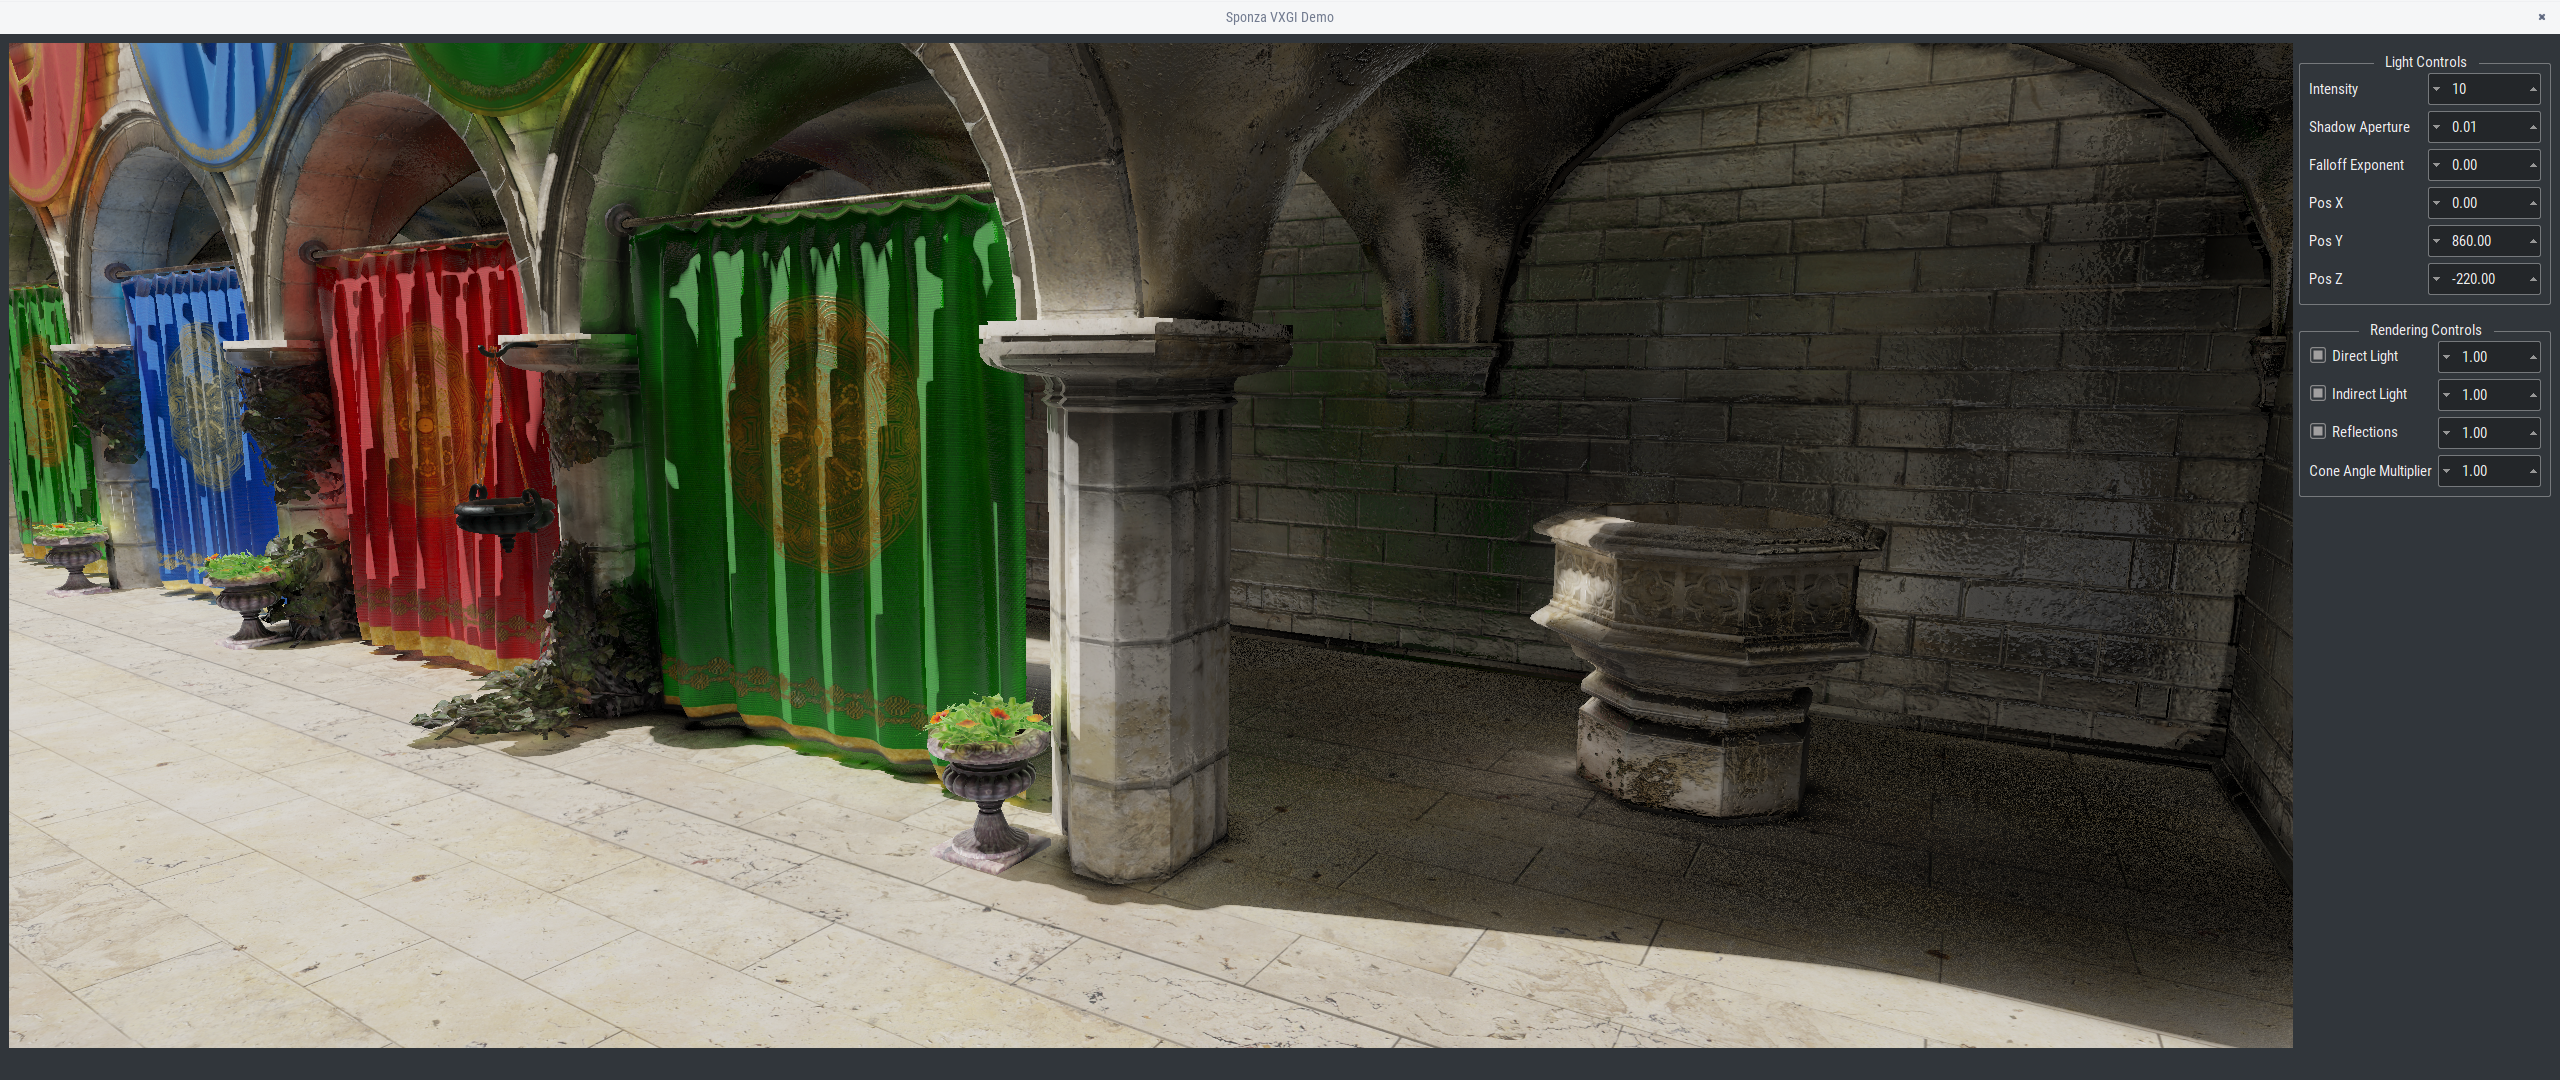
\includegraphics[width=1.0\linewidth]{images/full_render_01}
 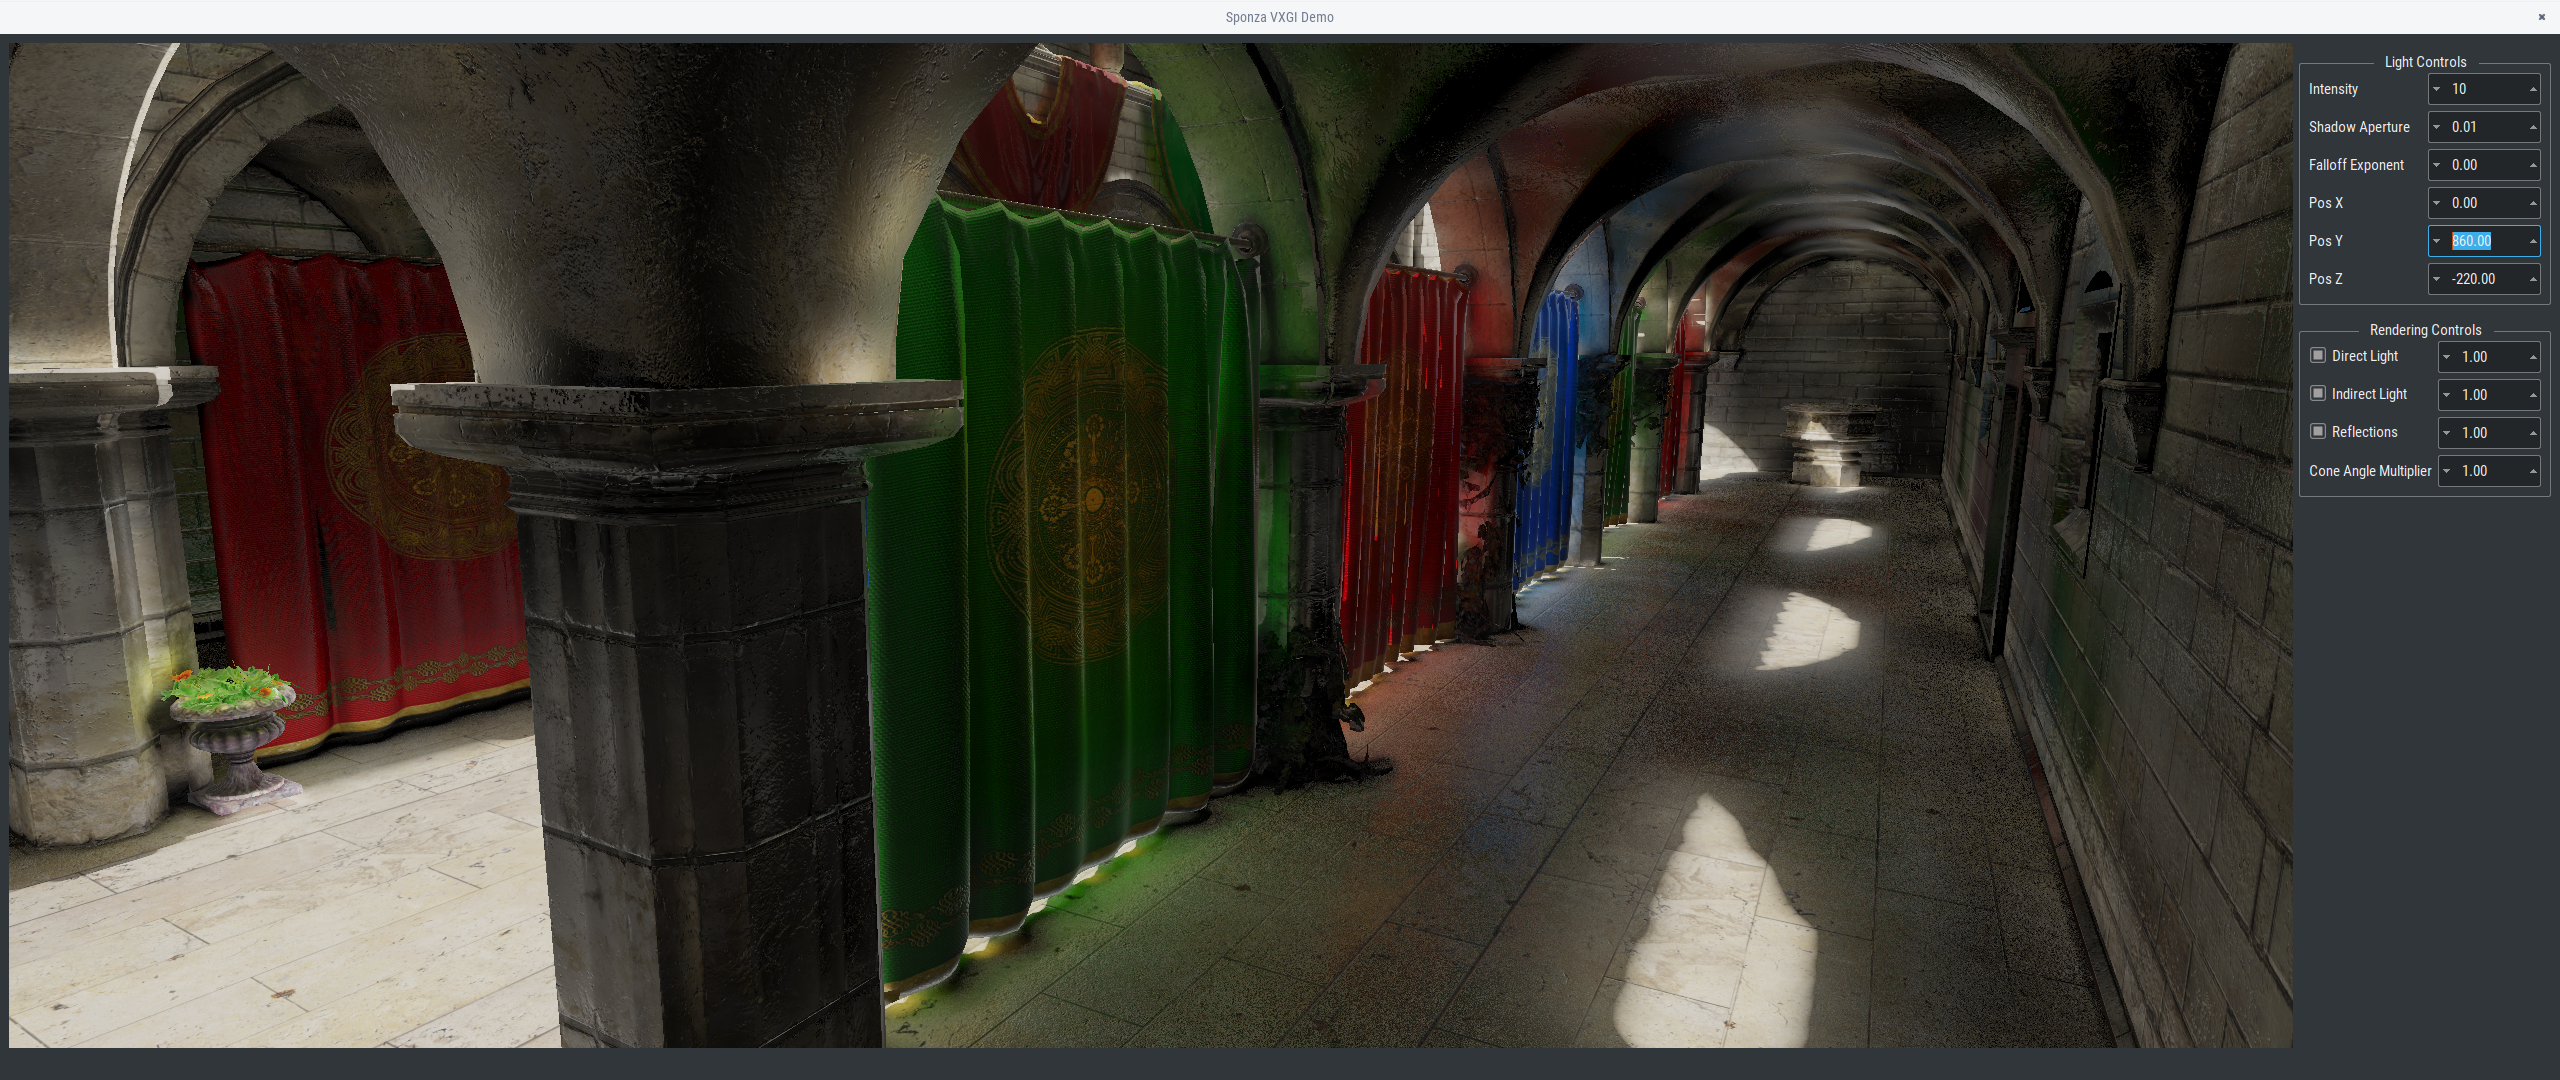
\includegraphics[width=1.0\linewidth]{images/full_render_02}
 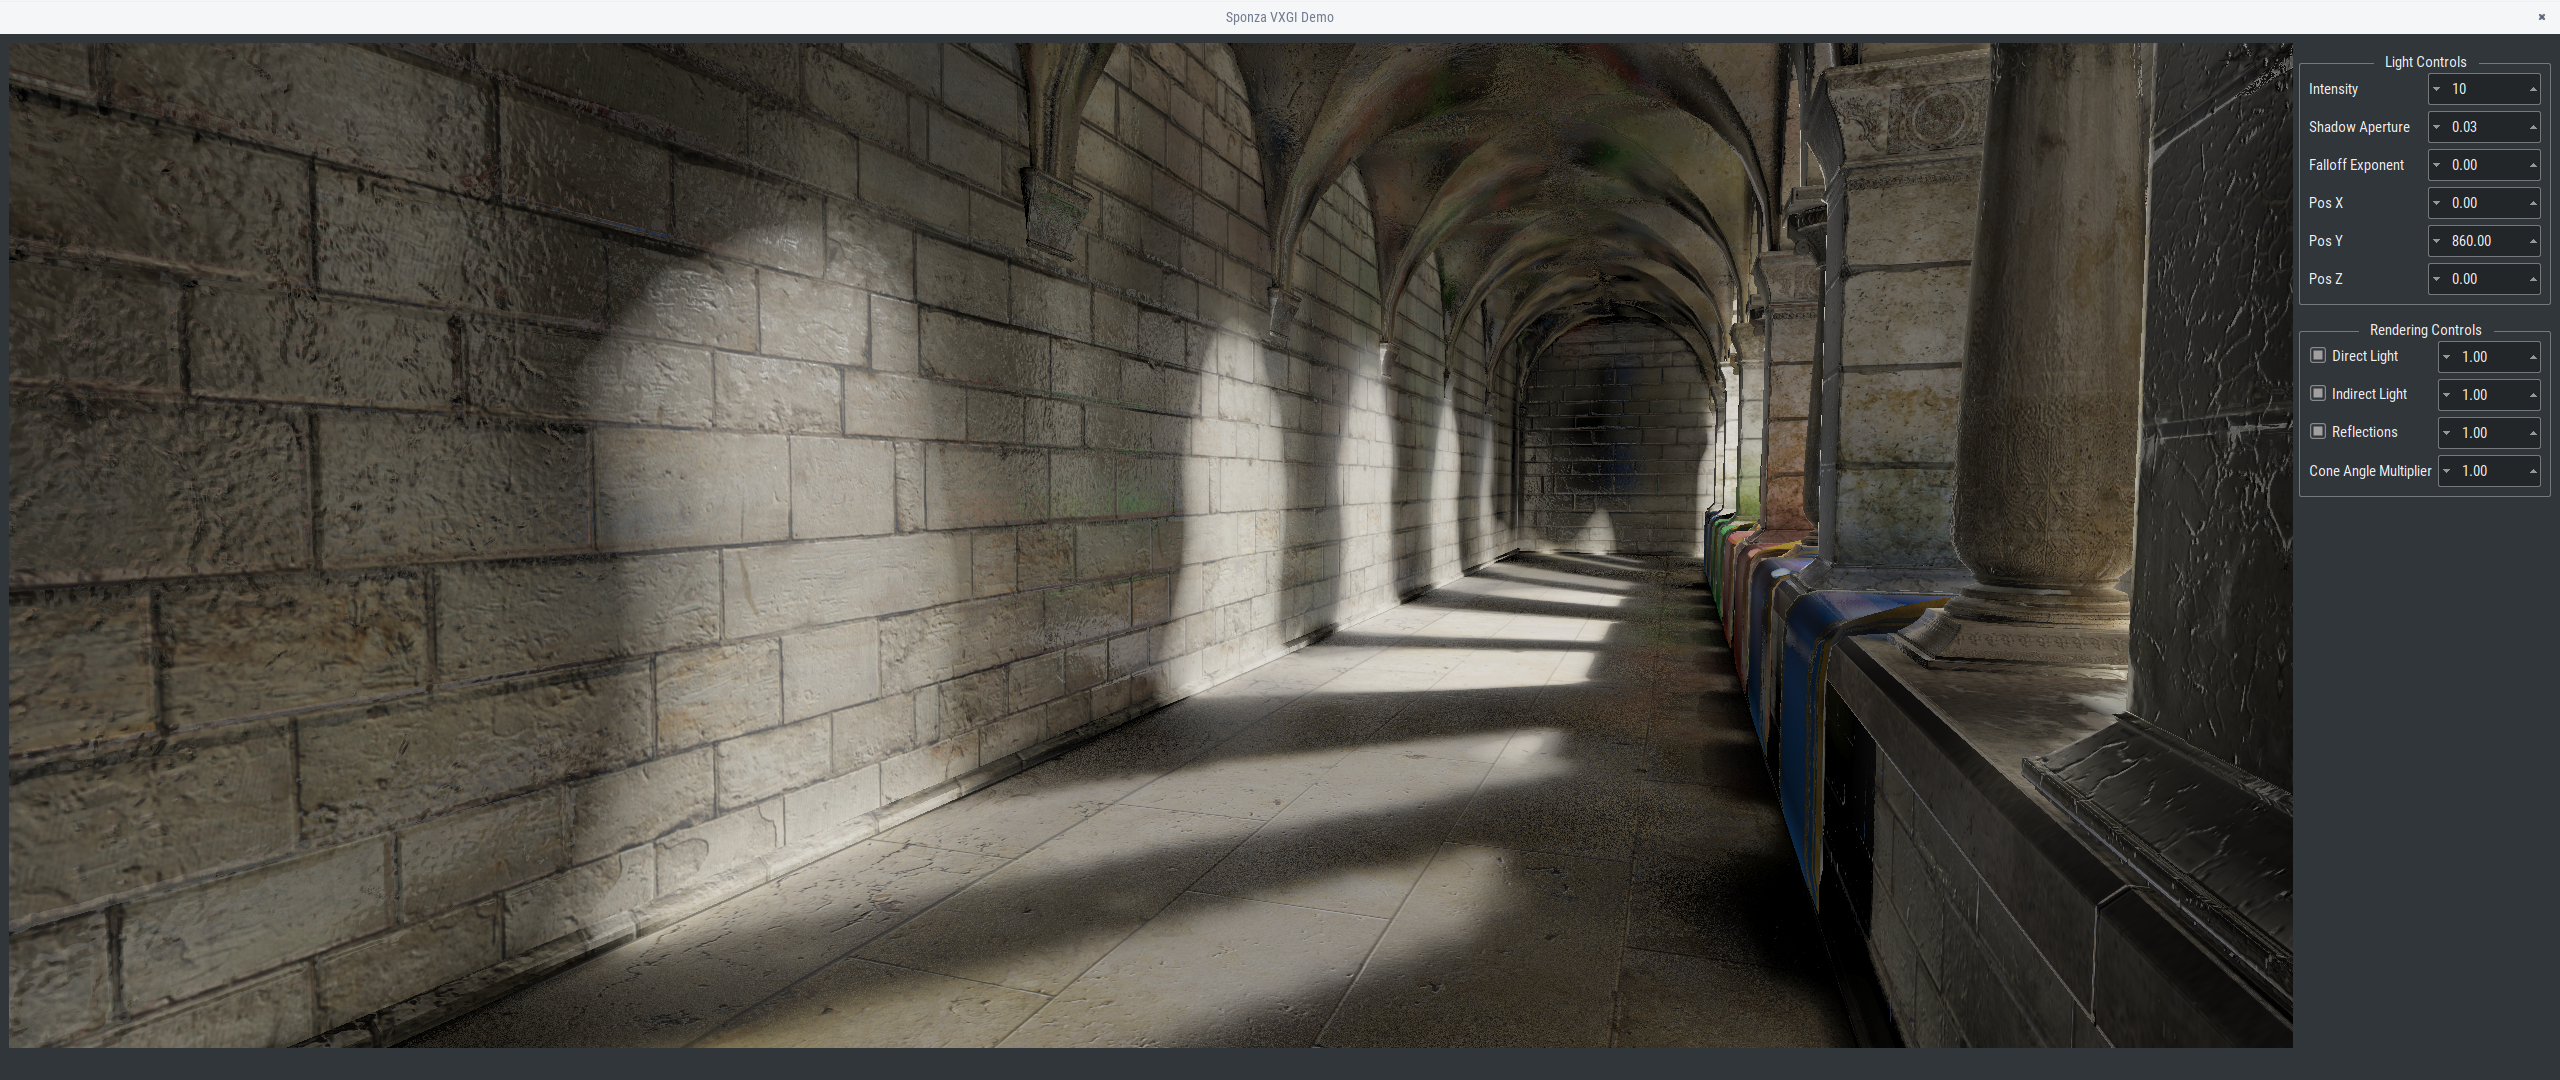
\includegraphics[width=1.0\linewidth]{images/full_render_03}
 \caption{\label{fig:reference}Three screenshots showing the full scene with a voxel resolution of $512^3$.}
\end{figure}

\begin{figure}[htbp]\centering
 \includegraphics[width=1.0\linewidth]{images/direct_only}
 \caption{A screenshot showing just the direct lighting pass.}
\end{figure}

\begin{figure}[htbp]\centering
 \includegraphics[width=1.0\linewidth]{images/indirect_only}
 \caption{A screenshot showing just the indirect lighting pass.}
\end{figure}

\begin{figure}[htbp]\centering
 \includegraphics[width=1.0\linewidth]{images/reflection_only}
 \caption{A screenshot showing just the reflection pass.}
\end{figure}

\begin{figure}[htbp]\centering
 \includegraphics[width=1.0\linewidth]{images/reflection_only_no_roughness}
 \caption{A screenshot showing just the reflection pass, but with the minimum cone angle.}
\end{figure}

\begin{figure}[htbp]\centering
\begin{center}
 \begin{tabular}{|c|c|c|c|}
 \hline
 Voxel Resolution & $256^3$ & $512^3$ & $768^3$ \\
 \hline
 \hline
 Frames per second & 60 & 60 & 60 \\
 \hline
 Memory usage & 1063MiB & 2615MiB & 6628MiB \\
 \hline
 Voxelisation & 2ms & 2ms & 2ms \\
 \hline
 Light Injection & 65ms & 378.5ms & 12294.5ms\\
 \hline
 Shading & 4.5ms & 4.5ms & 4.5ms \\
 \hline
 \end{tabular}
 \caption{\label{figure:performance} Averaged performance results when running with a NVIDIA GTX 1080 8GB at 2560x1080.}
\end{center}
\end{figure}

\section{Future Improvements}

Unfortunately I wasn't able to implement a sparse data structure as described in the source material \cite{crassinneyretsainzgreeneisemann2011} before the assignment deadline. Having a sparse data structure to store the emissive voxel texture would save a significant amount of GPU memory consumption, allowing the resolution for voxelization to be much higher; currently with dense 3D textures it is capable of exceeding both the 2 gigabyte memory limit of my GPU, and the 8 gigabyte limit of those at university.

The speed at which lighting rays are marched during the light injection pass would also be improved, as it would be able to step further through the voxel texture whilst ray marching if the higher levels in the octree are known to be empty.

I did start working on a sparse voxel octree as described in OpenGL Insights \cite{crassingreen2012} by using an OpenGL Atomic Counter for calculating the number of fragments needed for the voxel fragment list, and I believe I understand the technique well enough should I wish to implement it in the future.

The source material \cite{crassinneyretsainzgreeneisemann2011} also describes a method for anisotropic mip-mapping of the 3D texture, storing a version of the texture for each directional axis, which improves visual accuracy when cone tracing. Whilst I could have implemented this with the dense 3D textures I was using, I opted to use OpenGL's built in mip-mapping to save time.

\begin{figure}[htbp]\centering
 \includegraphics[width=1.0\linewidth]{images/banding.png}
 \caption{A screenshot showing banding artefacts in the reflection pass.}
\end{figure}

\begin{figure}[htbp]\centering
 \includegraphics[width=1.0\linewidth]{images/indirect_noise.png}
 \caption{A screenshot showing noise in the indirect lighting.}
\end{figure}

\begin{figure}[htbp]\centering
 \includegraphics[width=1.0\linewidth]{images/voxelization_error.png}
 \caption{A screenshot showing voxelization artefacts.}
\end{figure}

\bibliographystyle{acmsiggraph}
\bibliography{references}

\end{document}

